% Outline map for the PhD defense deck. One source, eight renders: the full map
% plus one focused variant per section.
% Compile: see build.sh in this directory (it prepares the badge images in
% .cache/, sets \focus and renames the output).
%
% Layout: Introduction, then the three ways we probe the Universe (CMB, weak
% lensing, statistical inference) down the left column, my two contributions
% down the middle, the conclusion on the right; arrows give the reading order.
% Each box carries small illustrated badges.
%
% \focus selects the highlighted box (0 = none, 1..7 = the sections). The
% geometry never moves between variants: only the opacity of the other boxes
% changes, so the SVGs register 1:1 inside the deck's .rail-stack.
\documentclass[tikz,border=2pt]{standalone}
\usepackage[utf8]{inputenc}
\usepackage{graphicx}
\usetikzlibrary{arrows.meta,calc,decorations.pathreplacing,shapes.geometric}

\providecommand{\focus}{0}

% Deck palette (keep in step with _common.py / phd.scss)
\definecolor{introtop}{HTML}{DDF0E6}\definecolor{introbot}{HTML}{A9D9BF}\definecolor{introline}{HTML}{2AA198}
\definecolor{obstop}{HTML}{E3ECF8}\definecolor{obsbot}{HTML}{A9C3E6}\definecolor{obsline}{HTML}{3B6FB6}
\definecolor{conttop}{HTML}{F1E4F2}\definecolor{contbot}{HTML}{D8A9D6}\definecolor{contline}{HTML}{521463}
\definecolor{ink}{HTML}{2E2E2E}
\definecolor{greytx}{HTML}{6E6E6E}
\definecolor{bracket}{HTML}{9A9A9A}

\newcommand{\boxw}{4.4}
\newcommand{\boxh}{1.55}

% Faded unless this index is focused, or nothing is: only \fv (opacity) changes,
% so every variant overlays the full map exactly. \sv (scale) and \wv (outline
% width) stay fixed. TikZ options cannot hold \ifnum.
\newcommand{\setlook}[1]{%
  \def\fv{0.32}\def\sv{1}\def\wv{0.8pt}%
  \ifnum\focus=0 \def\fv{1}\fi
  \ifnum\focus=#1 \def\fv{1}\fi}
\ifnum\focus=0 \def\av{1}\else \def\av{0.45}\fi

% #1 index  #2 name  #3 x  #4 y  #5 top  #6 bottom  #7 line  #8 label
\newcommand{\sectionbox}[8]{%
  \setlook{#1}%
  \begin{scope}[opacity=\fv,transparency group]
    \node[draw=#7,line width=\wv,top color=#5,bottom color=#6,
          rounded corners=6pt,minimum width=\boxw cm,minimum height=\boxh cm,
          align=center,text=ink,font=\sffamily\large,
          scale=\sv,transform shape] (#2) at (#3,#4) {#8};
  \end{scope}}

% A plain illustration or logo, faded with its box.
% #1 index  #2 x  #3 y  #4 \includegraphics...
\newcommand{\badge}[4]{%
  \setlook{#1}%
  \begin{scope}[opacity=\fv,transparency group]
    \node[inner sep=0] at (#2,#3) {#4};
  \end{scope}}

\tikzset{flow/.style={-{Stealth[length=6pt]},line width=0.9pt,greytx}}

\begin{document}
\begin{tikzpicture}
\useasboundingbox (-1.6,-9.8) rectangle (19.8,1.3);

% ---------------------------------------------------------------- boxes
\sectionbox{1}{intro}{3}{0}{introtop}{introbot}{introline}{Introduction}
\sectionbox{2}{cmb}{3}{-2.5}{obstop}{obsbot}{obsline}{The Cosmic Microwave\\Background}
\sectionbox{3}{wl}{3}{-5.0}{obstop}{obsbot}{obsline}{Weak Lensing}
\sectionbox{4}{stats}{3}{-7.5}{obstop}{obsbot}{obsline}{Statistical Inference}
\sectionbox{5}{c1}{10}{-3.2}{conttop}{contbot}{contline}{Component Separation}
\sectionbox{6}{c2}{10}{-6.6}{conttop}{contbot}{contline}{Field-Level Inference\\for Weak Lensing}
\sectionbox{7}{concl}{17.4}{-4.9}{introtop}{introbot}{introline}{Conclusion}

% ---------------------------------------------------------------- arrows
\begin{scope}[opacity=\av]
  \draw[flow] (3,-0.78) -- (3,-1.72);
  \draw[flow] (3,-3.28) -- (3,-4.22);
  \draw[flow] (3,-5.78) -- (3,-6.72);
  \draw[flow] (5.2,-7.5) .. controls (7.4,-7.5) and (6.7,-3.2) .. (7.75,-3.2);
  \draw[flow] (10,-3.98) -- (10,-5.82);
  \draw[flow] (12.2,-6.6) .. controls (13.9,-6.6) and (13.5,-4.9) .. (15.15,-4.9);
\end{scope}

% ---------------------------------------------------------------- brackets
\begin{scope}[opacity=\av]
  \draw[decorate,decoration={brace,amplitude=8pt,mirror},bracket,line width=0.9pt]
        (0.35,-1.6) -- (0.35,-8.4);
  \node[rotate=90,font=\sffamily\large,text=greytx] at (-0.55,-5.0)
        {How to probe the Universe};
  \draw[decorate,decoration={brace,amplitude=8pt},bracket,line width=0.9pt]
        (7.6,-1.25) -- (12.4,-1.25);
  \node[font=\sffamily\large,text=greytx] at (10,-0.5) {My contributions};
\end{scope}

% ---------------------------------------------------------------- badges
% Illustrations to the right of the probe boxes; the contributions' logos sit
% just above their box (SciPol: component separation; CosmoStat + AstroDeep:
% FLI, either side of the arrow), and the FLI pipeline sits under its box.
\badge{2}{5.75}{-2.5}{\includegraphics[height=1.55cm]{.cache/lcdm_cmb.pdf}}
\badge{3}{5.75}{-5.0}{\includegraphics[height=1.55cm]{.cache/lcdm_lss.pdf}}
\badge{4}{6.35}{-7.55}{\includegraphics[width=2.2cm]{.cache/mle_vs_bayes_icon.pdf}}
\badge{5}{12.95}{-3.2}{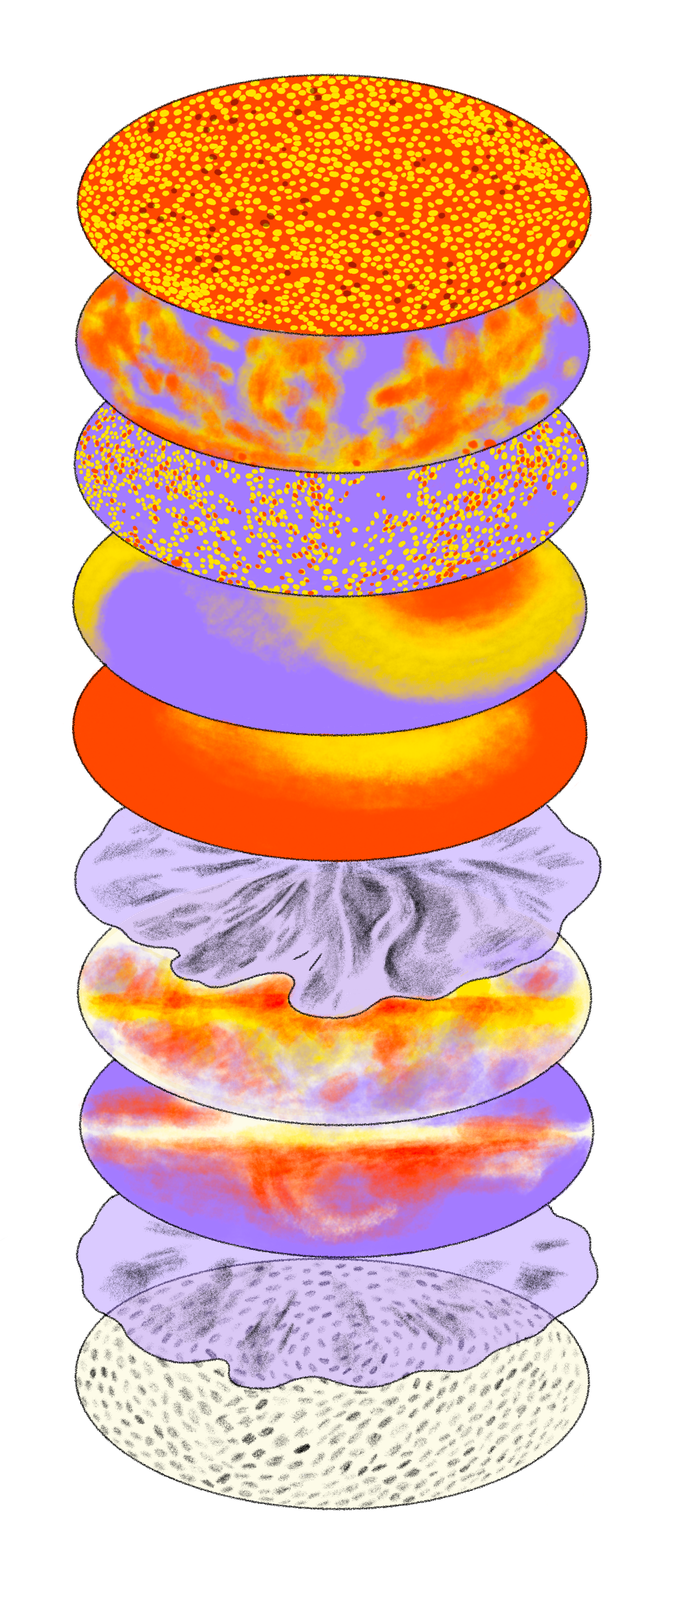
\includegraphics[height=1.95cm]{../3_observation/cmb/scipol/scipol_cmb_layers.png}}
\badge{5}{11.2}{-1.9}{\includegraphics[height=1.25cm]{../../Logos/scipol.png}}
\badge{6}{8.75}{-5.3}{\includegraphics[height=0.65cm]{../../Logos/cosmostat.png}}
\badge{6}{11.1}{-5.3}{\includegraphics[height=1.35cm]{../../Logos/AstroDeep-2.png}}
\badge{6}{10.0}{-8.6}{\includegraphics[width=3.0cm]{.cache/fli_pipeline.pdf}}
\end{tikzpicture}
\end{document}
